
\chapter{Implementierung}
\label{chapter-implementierung}
Das folgende Kapitel beschreibt die Implementierung des Backends,
Reservierungsinterfaces sowie des Fontends. Zunächst wird die Implementierung
des Reservierungsinterfaces und die damit einhergehende technischen Aspekten
beschreiben. Bei wird aufschluss über die Struktur gegben und die
Kernfunktionalität sowie Sackgassen in der Realisierung werden näher erläutert.
Daraufhin wird die Umsetzung des Frontend beschreiben. Abschließend wird auf die
Inbetriebnahme des Systems eingegangen.


\section{Implementierung des Reservierungsinterfaces}
Der Abschnitt beschreibt die Struktur des Reservierungsinterface mit seinen
technischen Aspekten und die Implementierung der Funktionalitäten
(\ref{section:funktionale}). Zunächst wird die Implementierung der
Kernfunktionalitäten erläutert. Daraufhin werden Sackgassen thematisiert.


\subsection{Struktur des Reservierungsinterface}
Das folgende Unterkapitel geht auf die Strukturen und Teilkomponenten des
Reservierungsinterface ein. In \ref{fig:db} wird die Verzeichnisstruktur
präsentiert. Das Reservierungsinterface teilt sich in drei wesentliche
Bausteine: \textit{node, SQLit(prisma)} und \textit{server.ts} .

\begin{figure}[h]
  \centering
  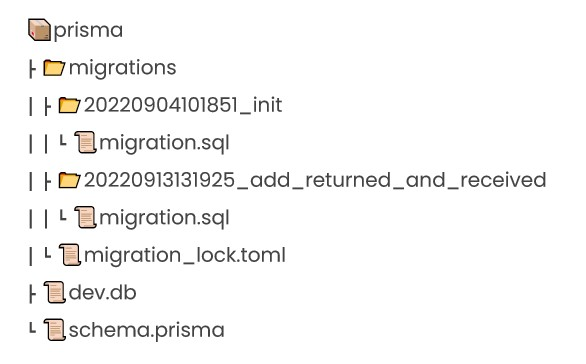
\includegraphics[scale=0.7]{Bilder/Db.jpg}
  \caption[Verzeichnisstruktur des Reservierungsinterfaces]{Verzeichnisstruktur des Reservierungsinterfaces}
  \label{fig:db}
\end{figure}

Der \textit{node} Ordner gibt... .



\textit{server.ts} für Routen


Die für das Reservierungsinterface entwickelte api lässt sich in drei Bereiche teilen:
\textit{Assets}, \textit{Kategorien} und \textit{Reservierungen} (\ref{table:impl-backend-routes}).
Um ein Asset zu reservieren, wird eine POST-Anfrage an \textit{/reservation/id} abgeschickt. Für die
Anfrage in Snipe-IT wird wiederum eine \textit{/reservation/receive} POST-Anfrage gesendet.
\ref{fig:orm} stellt die mit \textit{prisma} entwickelte Datenbank als Object Relational Mapper
(ORM) mit folgendem Schema dar. \textit{User} können \textit{Reservierungen} aufgeben.


\begin{table}[h]
  \centering
  \caption{api des Reservierungsinterfaces}
  \begin{tabular}{lll}
    \arrayrulecolor{maincolor}\hline
    \sffamily\color{maincolor}Methode & \sffamily\color{maincolor}Route           & \sffamily\color{maincolor}Funktion             \\
    \arrayrulecolor{maincolor}\hline
      GET               & \textit{/assets}       & Erhalte alle Assets \\
      GET               & \textit{/assets/:id}   &
      Erhalte ein Asset mit der entsprechend ID                               \\
      GET               & \textit{/categories} &
      Erhalte alle Kategorien                                        \\
      GET               & \textit{/reservation} &
      Erhalte Reservierungen                                       \\
      POST              & \textit{/reservation}       &
      Erstellen Reservierung                                            \\
      POST              & \textit{/reservation/receive}       &
      Erstellen Reservierung                                           \\
      POST              & \textit{/reservation/return}       &
      Erstellen Reservierung                                                \\
      POST              & \textit{/reservation/id}       &
      Erstellen Erstellen Reservierung                                                \\
      DELETE            & \textit{/reservation/delete}   &
      Löschen Reservierungen                         \\
      PATCH               & \textit{/reservation/patch}   & Verändern Reservieurng       \\
    \arrayrulecolor{maincolor}\hline
  \end{tabular}
  \label{table:impl-backend-routes}
\end{table}

\begin{figure}[h]
  \centering
  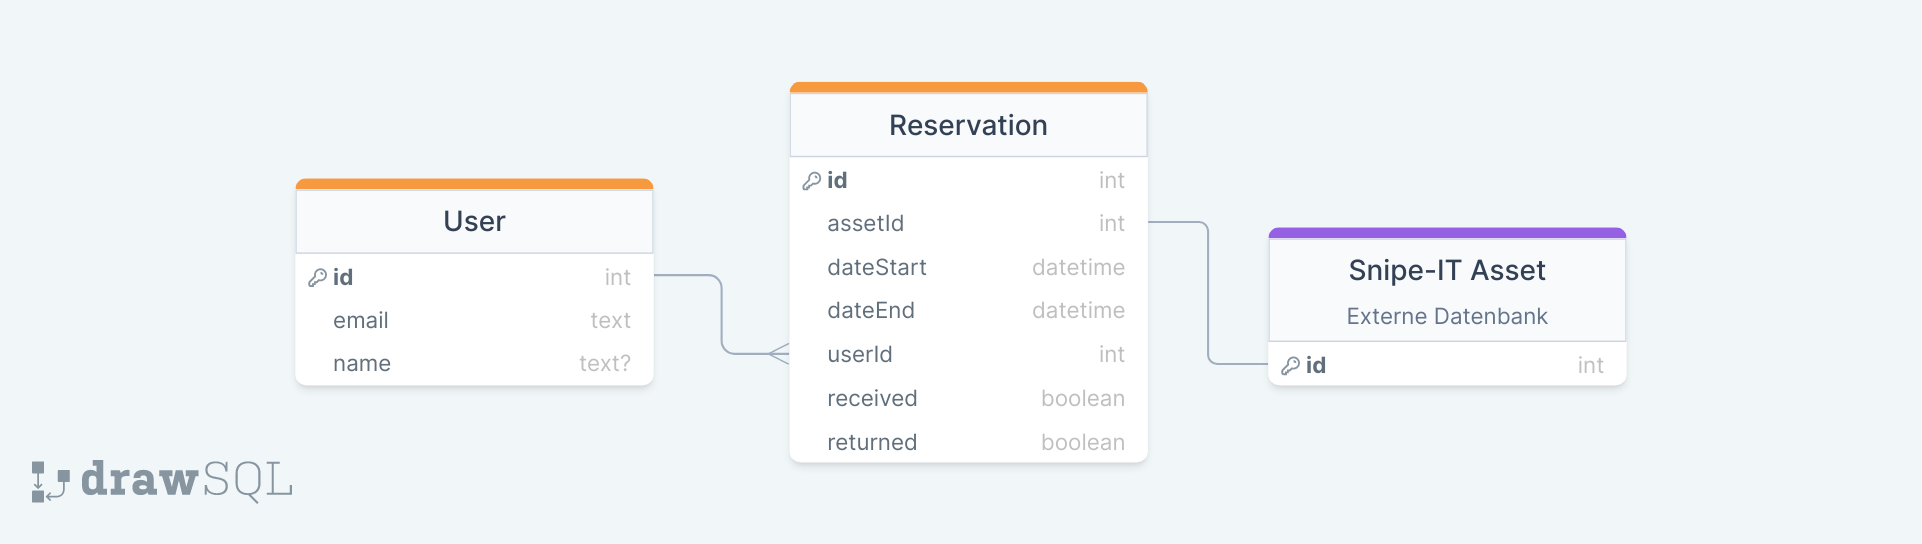
\includegraphics[scale=0.2]{Bilder/drawSQL-export-2022-10-09_15 56.png}
  \caption[Datenstruktur der Reservierungen in Verbindung mit Nutzenden]{Datenstruktur der Reservierungen in Verbindung mit Nutzenden}
  \label{fig:orm}
\end{figure}


\subsection{Implementierung der Kernfunktionalität}
Dieser Abschnitt präsentiert die Implementierung der Kernfunktionalität des
Zwischenbackends, welche aus den Anforderungen  bestimmt wurden
(\ref{section:anforderung}). Bei der Funktionalität handelt es sich um das
Reservieren in die Zukunft, sowie das Speichern dieser Vorgänge und die damit
einhergehende Bestätigung für die Aktualisierung in Snipe-IT.

Um auf die Assets zugreifen zu können wurde mit der Snipe-IT JSON REST API gearbeitet. Die snipe-it
api umfasst viele Befehle. Relevante Befehle für diese Arbeit waren \textit{/hardware,
/statuslabels, /users, /categories}. Mithilfe dieser konnten die Assets der Beispieldatenbank
genutzt werden. Ein /statuslabel ist im ausgeliehenen zustand immer an einen /user gebunden.
\ref{fig:snipe} zeigt einen Ausschnitt der Komplexität und der Möglichkeiten, die die api bietet.

\begin{figure}[h]
  \centering
  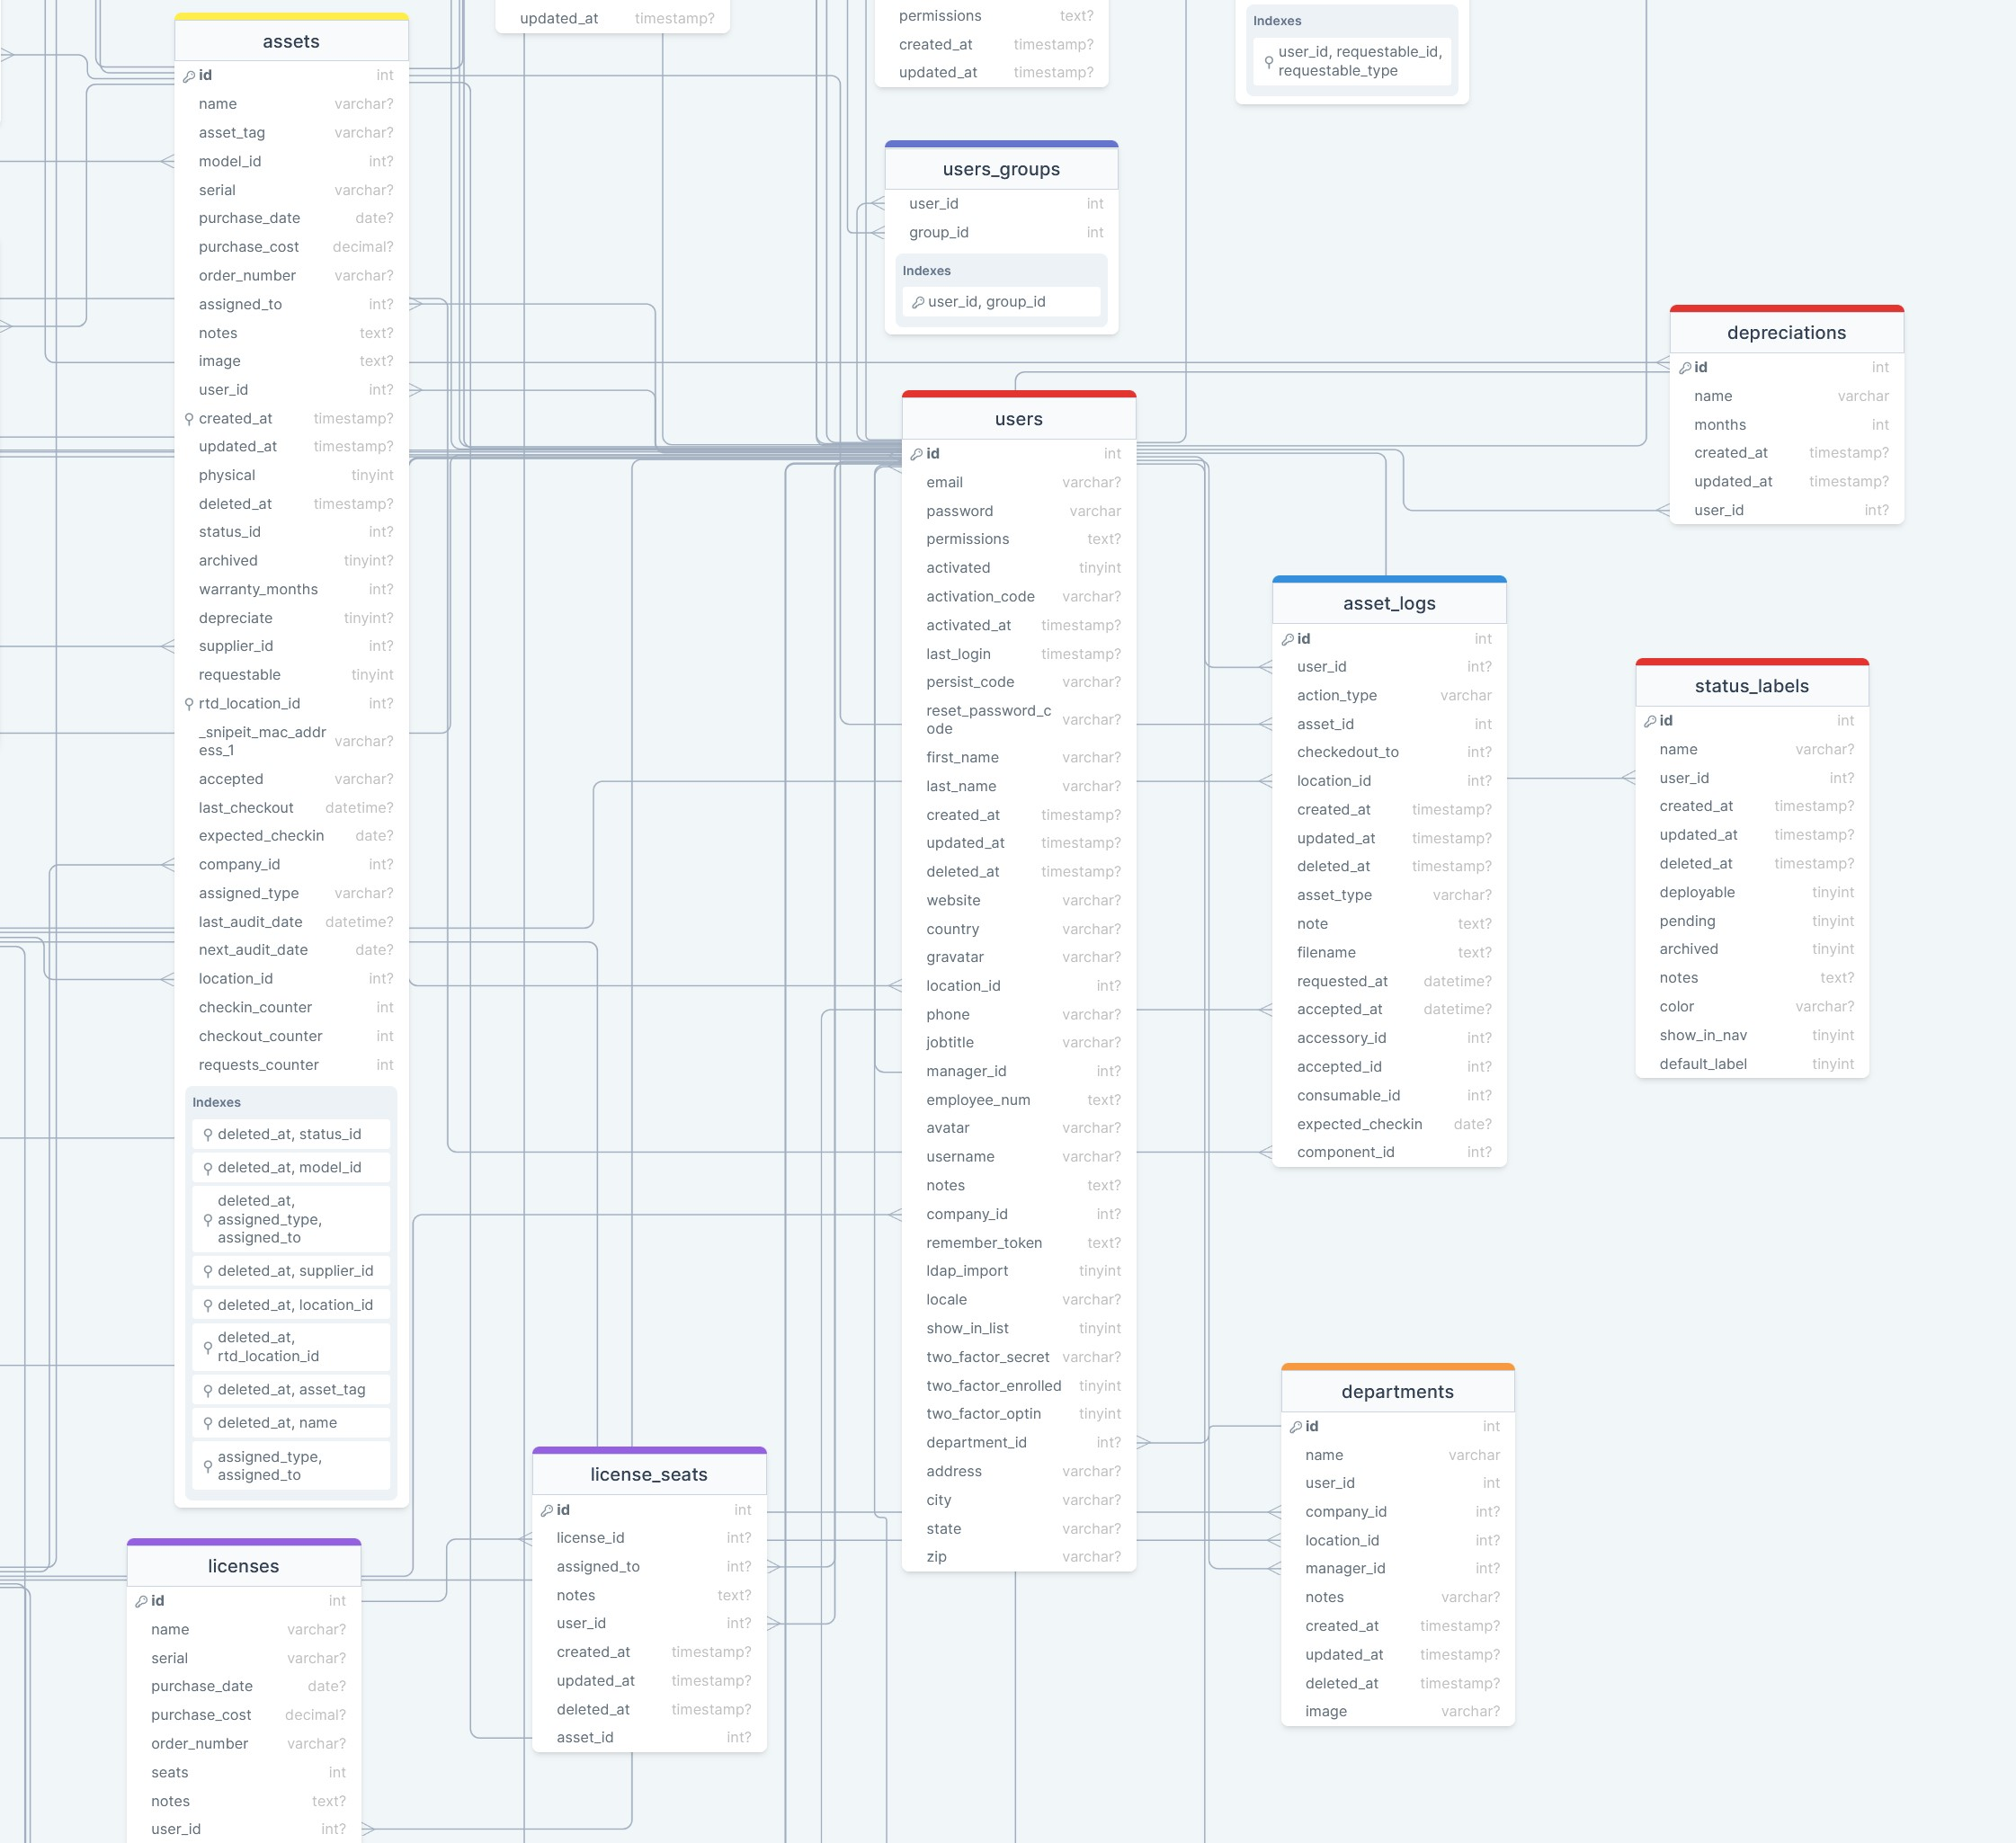
\includegraphics[scale=0.3]{Bilder/snipe.jpg}
  \caption[UML Snipe-IT api]{UML Snipe-IT api}
  \label{fig:snipe}
\end{figure}

Um mit der api arbeiten zu können muss ein \textit{API
  key}\footnote{\url{https://snipe-it.readme.io/reference/generating-api-tokens}}
  generiert werden. Da persönliche Zugriffstoken verwendet werden, spiegeln die
  Berechtigungen des API-Tokens die Berechtigungen des Nutzenden wider. Das
  bedeutet auch, das die Token lediglich manuell im Dashboard generierbar sind.
  Was zur folge hat, dass das geplante LDAP-System der Universität zu Lübeck
  nicht ohne umstände eingebunden und entsprechend genutzt werden kann. Snipe-IT
  gibt unter anderem die Möglihkeit, das LDAP
  Formular\footnote{\url{https://snipe-it.readme.io/docs/ldap-sync-login}}
  einfach einzubinden, trotzdessen besteht das Problem, der Autentifizierung
  sowie generierung der Tokens offen, da die Daten im Reservierungsinterface bis
  dato nicht übertragen wurdne.


FÜR FRONTEND benötigte Ressourcen: Routen angelegt -> Fastify genutzt, für
vereinfachung


Reservierung in der Zukunft: Daten zwischenspeichern, weil Snipe IT doof ->
SQLite -> Prisma (für einfache verwaltung -> Beispeil und wie es Funktioniert)


Statuseingabe/Ausleihen schwer und komisch -> rumarbeiten

\section{Implementierung des Frontends}
Das kommende Unterkapitel beschreibt die Client-seitige Realisierung der Arbeit. Zunächst wird der
Aufbau betrachtet (\ref{fig:vue}), daraufhin wird die Nutzung von vue und XXX erläutert. Des Weiteren wird auf die
Struktur der Komponenten eingegangen (\ref{fig:komponenten}). Abschließend wird das native App-Erlebnis thematisiert.

\begin{figure}[h]
  \centering
  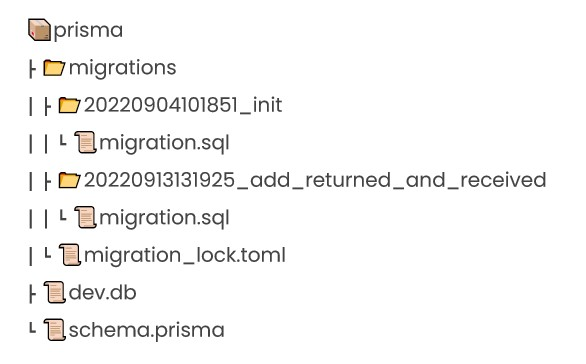
\includegraphics[scale=0.7]{Bilder/Db.jpg}
  \caption[Verzeichnisstruktur des Reservierungsinterfaces]{Verzeichnisstruktur des Reservierungsinterfaces}
  \label{fig:vue}
\end{figure}

Für den Aufbau des Projektes wurde vue.js verwendet. Um das Styling zu vereinfachen wurde
Tailwindcss verwendet. Die Kalenderkomponente wurde durch v-calender ergänzt. Der Kalender stellt
einen wichtigen Bestandteil für das Reservieren dar. Durch die Möglichkeiten der Komponente ...??.
Außerdem bietet diese viele Ausbaumöglichkeiten für folgende Funktionalitäten.

Um bessere Vorschläge in der Entwicklungsumgebung zu ermöglichen und vorzeitige Fehler zu minimieren
wurde ergänzt zu JavaScript TypeScript verwendet.



Bei der Implementierung wurde sich an den best practices der Vue.js-Dokumentation orientiert
\todo{(Vue.js, 2021a)}. Für sich wiederholende Elemente wurden eigene Views erstellt.

\begin{figure}[h]
  \centering
  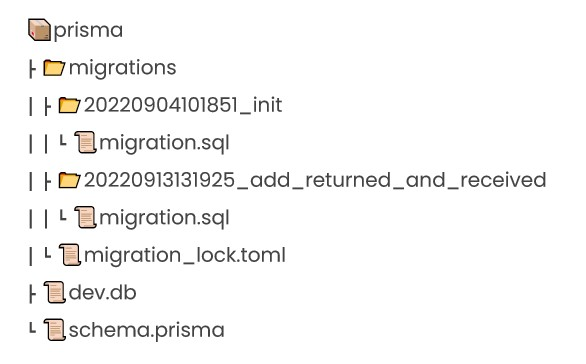
\includegraphics[scale=0.7]{Bilder/Db.jpg}
  \caption[Verzeichnisstruktur des Reservierungsinterfaces]{Verzeichnisstruktur des Reservierungsinterfaces}
  \label{fig:Komponenten}
\end{figure}




\begin{itemize}
  \item Preline für UI -> Nicht empfehlenswert (Sackgassen)
  \item Headless ui für animation
  \item 
\end{itemize}

Aufteilung mit dem Bindestrich: Kategorien im Frontend

\begin{lstlisting}
fetch(import.meta.env.VITE_SERVER_URL + "/categories", options)
.then(res => res.json())
.then(data => (categories.value = data.categories.rows))
.then(() => {
	categories.value = categories.value
		.map(category => {
			const catSplit = category.name.split(" - ");
			return {
				id: category.id,
				category: catSplit[0],
				subcategory: catSplit[1],
			};
		})
		.reduce((acc, category) => {
			return {
				...acc,
				[category.category]: [
					...(acc[category.category] ?? []),
					{
						id: category.id,
						subcategory: category.subcategory,
					},
				],
			};
		}, {});
\end{lstlisting}




\section{Nutzung des Systems}
Der folgende Abschnitt führt die nötigen Schritte auf, um das System in Betrieb
nehmen zu können. Zuerst wird die Installation erklärt, gefolgt von der Konfiguration und Ausführung
des Systems. 

\subsection{Installation}
Für die Nutzung des Systemes wird eine Installation von \textit{Node.js} sowie der Paket-Manager
\textit{npm} benötigt. Anschließend, kann das System auf\dots

\subsection{Konfiguration}


\subsection{Ausführung von Snipe-IT}
Um das System Nutzen und weiterentwicklen zu können muss... API KEy generieren
lassen.

\subsection{Ausführung der Web-App}



\section{Fazit der Implementierung}

Sackgassen YEAH
